This search aims to look for charged particles decaying inside the tracker to one fermion and a neutralino. 
In case the chargino and the lightest neutralino are almost mass-degenerate the fermion is very low in momentum and can therefore be hardly detected in the tracker. 
The momentum of the fermion is of course highly dependent on the actual mass gap between the neutralino and the chargino. 
The typical \pt distribution of a pion when the mass gap is about the pion mass is shown in figure \ref{bla bla}
\begin{figure}[!tp]
  \centering 
  \begin{tabular}{c}
    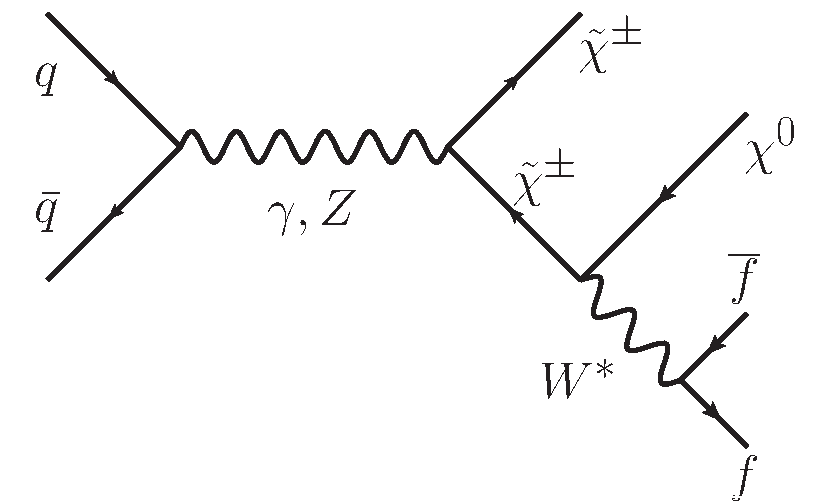
\includegraphics[width=0.85\textwidth]{figures/CharginoPairProductionDiagrams_Decay.pdf}
  \end{tabular}
  \caption{Feynman diagram showing production and decay of a chargino pair.}
  \label{fig:feynmanDiagram}
\end{figure}
\begin{figure}[!tp]
  \centering 
  \begin{tabular}{c}
    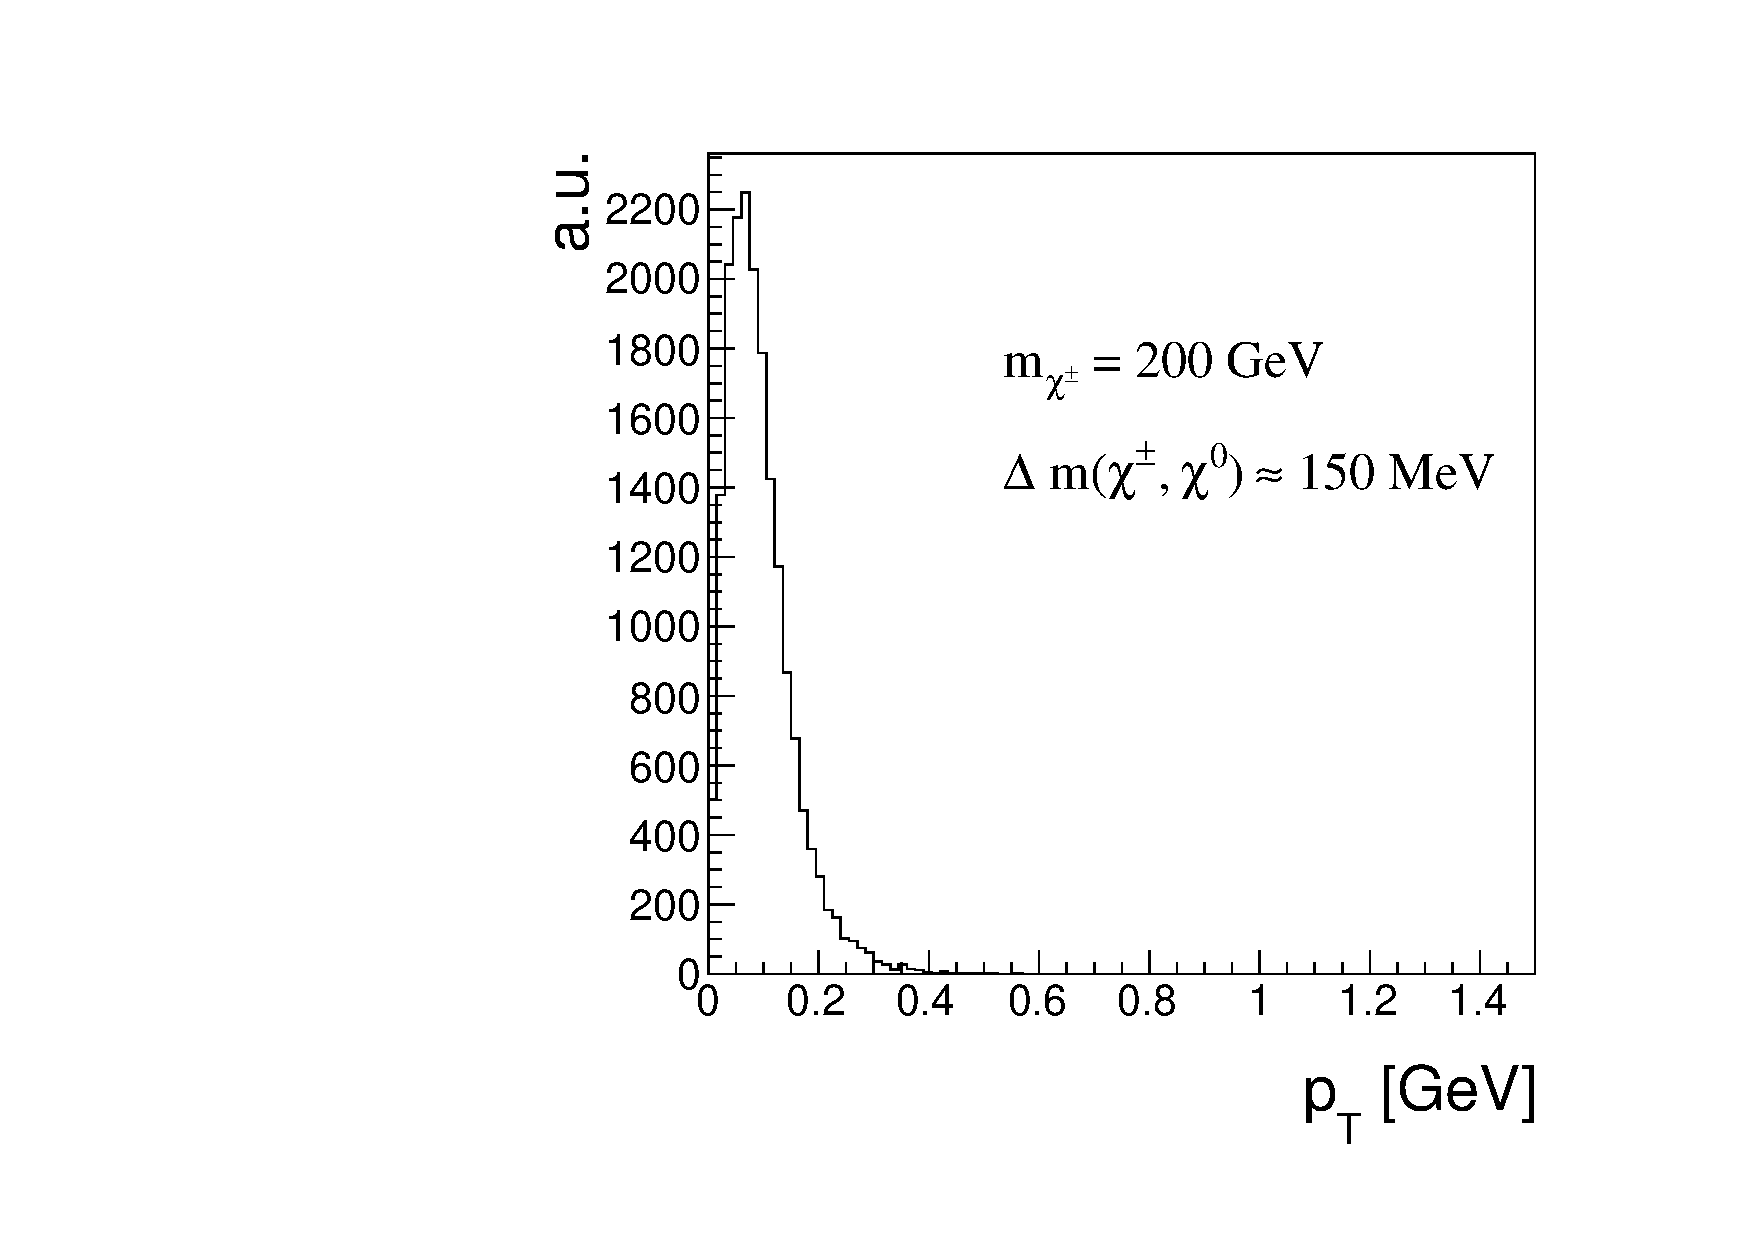
\includegraphics[width=0.85\textwidth]{figures/ptOfPions.pdf}
  \end{tabular}
  \caption{Transverse momentum distribution of pions coming from chargino decay into a neutralino with a mass gap of 150\mev.}
  \label{fig:ptOfPions}
\end{figure}
Being in principle sensitive to any physics beyond the standard model, this search is motivated by the possible existence of a supersymmetric chargino.
As showed in chaper \ref{bla} Supersymmetry is one of the most promising theories beyond the Standard Model and is very well motivated from either theoretical and experimental point of view. 
It is  able to give possible answers to the main short-comings of th SM and is therefore an attractive theory, which deserves to be looked at.

There are many analyses done at CMS which are in principle sensitive to such a supersymmetric chargino. 
This analyis wants to focus on long lifetimes such that the chargino does not directly decay, but reaches at least to first layers of the detector, being the silicon pixel and strip trackers. 
On the other hand, it has been designed in a way, that the chargino is not that-lonmg lived, that it travels through the whole detector, but decays at least before the muon chambers, thus is not reconstructed as a muon.
There have been analysis at CMS and Atlas looking for such middel-live charginos. 
The new aspect of the analysis is the inclusion of the variable dE/dx.
The pixel and the silicon tracker at CMS have been calibrated already offline, when building these moduls. Unfortunately it is not so good.
The silicon strip tracker has been calibrated in the context of a search for heavy, stable charged particle (cite something).
In this analysis, also very short tracks become very important, showing not more than three of four hits. Therfore also the pixel detector needs to bec calibrated in order to increase senssitivy for those short tracks

\section{General search strategy}
\begin{itemize}
\item Importance of De/Dx 
\item No cut on number of valid hits
\item Importance of pixel gain calibration
\end{itemize}

\section{Gain calibration of the silicon pixel tracker}
See small document I wrote.

\section{Signal samples}
\begin{itemize}
\item signal samples generated with Madgraph and pythia
\item They are decayed in Geant to only pions. Around ten different lifetimes were simulated
\item Higgsino/wino chargino 
\item append slha file
\item For other lifetimes: lifetime reweighting is done PLOT
\item For five diffenrent masses (100-500 GeV) 
\end{itemize}

\section{Event selection}

\section{Main discriminating variables}
\begin{itemize}
\item dE/dx
\item pt
\end{itemize}

\section{Sources of backgrounds}
\begin{itemize}
\item Background consist of particles which make high energy deposits and are high pt
\item In general: Low background search
\end{itemize}
\subsection{Fake tracks}
\begin{itemize}
\item Definition of fake tracks
\item How can they fake the signal
\end{itemize}
\subsection{Muons}
\begin{itemize}
\item How can muons fake the signal
\end{itemize}
\subsection{Pions}
\begin{itemize}
\item How can pions fake the signal
\end{itemize}
\subsection{Electrons}
\begin{itemize}
\item How can electrons fake the signal
\end{itemize}

\section{Background estimation methods}
\subsection{Fake background}
\subsection{Leptonic background}




\section{Optimisation of search sensitivity}
\begin{itemize}
\item Show plots
\item show table
\end{itemize}

\section{Systematic ucnertainties}
Obvious

\section{Results}
\begin{itemize}
\item Method of limit setting
\item 1-d limits
\item 2-d limits
\end{itemize}

